% answers.tex —— 2017 年·北京卷·理科 · 参考答案与详细解析片段
% 由 tools/generate_projects.py 依来源总账自 2017/2017_数学真题_北京理_试题.md + 2017/2017_数学真题_北京理_解析正文.md + 2017/2017_数学真题_北京理_答案要点.md 生成，勿手改（改源 MD 后重跑）


\begin{gknotice}
\textbf{解析归属}：固定来源仅含题面。以下由本库独立推导并经异人盲核，非官方解析；结论等级至多为 D。
\end{gknotice}

\begin{answer}
\gksolhead{1}{}

\textbf{题目}：

若集合 $A=\{x\mid -2<x<1\}$，$B=\{x\mid x<-1\text{ \text{或} }x>3\}$，则 $A\cap B=$（　）

\begin{itemize}
\item （A）$\{x\mid -2<x<-1\}$
\item （B）$\{x\mid -2<x<3\}$
\item （C）$\{x\mid -1<x<1\}$
\item （D）$\{x\mid 1<x<3\}$
\end{itemize}

\Needspace{4\baselineskip}
\textbf{解析}

$A=(-2,1)$，而 $B=(-\infty,-1)\cup(3,+\infty)$。两者重叠部分只有 $(-2,-1)$，故选 \textbf{A}。

检查：两个端点都不属于交集，$x>3$ 的分支与 $A$ 无交；没有把并集当交集。

\gkanswer{答案：A}

\end{answer}
\begin{answer}
\gksolhead{2}{}

\textbf{题目}：

若复数 $(1-\mathrm i)(a+\mathrm i)$ 在复平面内对应的点在第二象限，则实数 $a$ 的取值范围是（　）

\begin{itemize}
\item （A）$(-\infty,1)$
\item （B）$(-\infty,-1)$
\item （C）$(1,+\infty)$
\item （D）$(-1,+\infty)$
\end{itemize}

\Needspace{4\baselineskip}
\textbf{解析}

\Needspace{5\baselineskip}
展开得

\nopagebreak[4]
\[
(1-\mathrm i)(a+\mathrm i)=(a+1)+(1-a)\mathrm i.
\]

第二象限要求 $a+1<0$ 且 $1-a>0$，合并为 $a<-1$，故选 \textbf{B}。

检查：$a=-1$ 时实部为零，落在坐标轴上，应排除；取 $a=-2$，得到 $-1+3\mathrm i$，确在第二象限。

\gkanswer{答案：B}

\end{answer}
\begin{answer}
\gksolhead{3}{}

\textbf{题目}：

执行如图所示的程序框图，输出的 $S$ 值为（　）
\nopagebreak[4]
\begin{center}\begin{tikzpicture}[>=stealth,thick,
  term/.style={draw,rounded corners=3pt,minimum width=22mm,minimum height=7mm},
  proc/.style={draw,minimum width=30mm,minimum height=8mm,align=center},
  test/.style={draw,diamond,aspect=2.2,inner sep=1pt,align=center},
  io/.style={draw,trapezium,trapezium left angle=70,trapezium right angle=110,
    minimum width=27mm,minimum height=8mm,align=center}]
  \node[term] (start) at (-2,0) {开始};
  \node[proc] (init) at (-2,-1.15) {$k=0,\ s=1$};
  \node[test] (test) at (0,-2.65) {$k<3$？};
  \node[proc] (inc) at (3,-2.65) {$k=k+1$};
  \node[proc] (update) at (3,-1.15) {$s=\dfrac{s+1}{s}$};
  \node[io] (out) at (0,-4.15) {输出 $s$};
  \node[term] (stop) at (0,-5.25) {结束};
  \draw[->] (start)--(init);
  \draw[->] (init)--(test);
  \draw[->] (test.east)--node[above]{是}(inc.west);
  \draw[->] (inc.north)--(update.south);
  \draw[->] (update.west)--++(-1.05,0)|-(test.north);
  \draw[->] (test.south)--node[right]{否}(out.north);
  \draw[->] (out)--(stop);
\end{tikzpicture}
\end{center}
\nopagebreak[4]
\begin{itemize}
\item （A）$2$
\item （B）$\dfrac32$
\item （C）$\dfrac53$
\item （D）$\dfrac85$
\end{itemize}

\Needspace{4\baselineskip}
\textbf{解析}

按 F03 的箭头，先判断，成立时先令 $k=k+1$，再更新 $s$，然后返回判断。

\begin{center}
\begin{tabular}{lll}
\toprule
状态 & $k$ & $s$ \\
\midrule
初始化 & 0 & 1 \\
第一次循环后 & 1 & 2 \\
第二次循环后 & 2 & $3/2$ \\
第三次循环后 & 3 & $5/3$ \\
\bottomrule
\end{tabular}
\end{center}

此时 $k<3$ 不成立，输出 $5/3$，故选 \textbf{C}。

检查：恰执行三轮，所有参与除法的 $s$ 均非零；没有多执行一轮得到 $8/5$。题干 $S$ 与框图 $s$ 的大小写差异不影响框图执行结果。

\gkanswer{答案：C，$5/3$}

\end{answer}
\begin{answer}
\gksolhead{4}{}

\textbf{题目}：

\Needspace{5\baselineskip}
若 $x,y$ 满足

\nopagebreak[4]
\[
\begin{cases}
x\leqslant3,\\
x+y\geqslant2,\\
y\leqslant x,
\end{cases}
\]

则 $x+2y$ 的最大值为（　）

\begin{itemize}
\item （A）$1$
\item （B）$3$
\item （C）$5$
\item （D）$9$
\end{itemize}

\Needspace{4\baselineskip}
\textbf{解析}

\Needspace{5\baselineskip}
由 $y\leqslant x$ 及 $x\leqslant3$，

\nopagebreak[4]
\[x+2y\leqslant3x\leqslant9.\]

在 $(x,y)=(3,3)$ 时，三个限制 $x\leqslant3$、$x+y\geqslant2$、$y\leqslant x$ 均满足，且目标值为 $9$，故最大值是 $9$，选 \textbf{D}。

检查：上界可取到，不只是形式估计。可行域顶点为 $(1,1),(3,-1),(3,3)$，对应目标值 $3,1,9$，一致。

\gkanswer{答案：D，$9$}

\end{answer}
\begin{answer}
\gksolhead{5}{}

\textbf{题目}：

已知函数 $f(x)=3^x-\left(\dfrac13\right)^x$，则 $f(x)$（　）

\begin{itemize}
\item （A）是奇函数，且在 $\mathbb R$ 上是增函数
\item （B）是偶函数，且在 $\mathbb R$ 上是增函数
\item （C）是奇函数，且在 $\mathbb R$ 上是减函数
\item （D）是偶函数，且在 $\mathbb R$ 上是减函数
\end{itemize}

\Needspace{4\baselineskip}
\textbf{解析}

\Needspace{5\baselineskip}
定义域为 $\mathbb R$，$f(x)=3^x-3^{-x}$，故

\nopagebreak[4]
\[f(-x)=3^{-x}-3^x=-f(x).\]

\Needspace{5\baselineskip}
又

\nopagebreak[4]
\[f'(x)=\ln3\,(3^x+3^{-x})>0\qquad(x\in\mathbb R).\]

因此为奇函数且在 $\mathbb R$ 上严格递增，选 \textbf{A}。

检查：定义域关于原点对称，$f(0)=0$；导数第二项符号为正。

\gkanswer{答案：A}

\end{answer}
\begin{answer}
\gksolhead{6}{}

\textbf{题目}：

设 $\boldsymbol m,\boldsymbol n$ 为非零向量，则“存在负数 $\lambda$，使得 $\boldsymbol m=\lambda\boldsymbol n$”是“$\boldsymbol m\cdot\boldsymbol n<0$”的（　）

\begin{itemize}
\item （A）充分而不必要条件
\item （B）必要而不充分条件
\item （C）充分必要条件
\item （D）既不充分也不必要条件
\end{itemize}

\Needspace{4\baselineskip}
\textbf{解析}

\Needspace{5\baselineskip}
若 $\boldsymbol m=\lambda\boldsymbol n$ 且 $\lambda<0$，则

\nopagebreak[4]
\[\boldsymbol m\cdot\boldsymbol n=\lambda|\boldsymbol n|^2<0,\]

故前者是后者的充分条件。

反之，取 $\boldsymbol m=(1,0)$、$\boldsymbol n=(-1,1)$，内积为 $-1<0$，但两向量不共线，不存在使 $\boldsymbol m=\lambda\boldsymbol n$ 成立的实数 $\lambda$。所以不必要，选 \textbf{A}。

检查：反例中两向量都非零，符合题设。

\gkanswer{答案：A}

\end{answer}
\begin{answer}
\gksolhead{7}{}

\textbf{题目}：

某四棱锥的三视图如图所示，则该四棱锥的最长棱的长度为（　）
\nopagebreak[4]
\begin{center}\begin{tikzpicture}[thick,>=stealth,line cap=round,line join=round,
  dim/.style={<->,thin}, every node/.style={font=\small}]
  % Front view: right triangle with horizontal and vertical legs both 2.
  \draw (0,0)--(2.4,0)--(2.4,2.4)--cycle;
  \draw[dim] (0,-.42)--(2.4,-.42) node[midway,below]{2};
  \draw[thin] (0,-.12)--(0,-.52) (2.4,-.12)--(2.4,-.52);
  \draw[dim] (2.82,0)--(2.82,2.4) node[midway,right]{2};
  \draw[thin] (2.52,0)--(2.92,0) (2.52,2.4)--(2.92,2.4);
  \node at (1.2,2.85) {正视图};
  % Side view: square face and its visible diagonal.
  \draw (5,0) rectangle (7.4,2.4);
  \draw (5,0)--(7.4,2.4);
  \draw[dim] (5,-.42)--(7.4,-.42) node[midway,below]{2};
  \draw[thin] (5,-.12)--(5,-.52) (7.4,-.12)--(7.4,-.52);
  \node at (6.2,2.85) {侧视图};
  % Plan view: right triangle and its internal diagonal.
  \draw (0,-3.15)--(2.4,-3.15)--(2.4,-5.55)--cycle;
  \draw (0,-3.15)--(2.4,-5.55);
  \node at (1.2,-5.95) {俯视图};
\end{tikzpicture}
\end{center}
\nopagebreak[4]
\begin{itemize}
\item （A）$3\sqrt2$
\item （B）$2\sqrt3$
\item （C）$2\sqrt2$
\item （D）$2$
\end{itemize}

\Needspace{4\baselineskip}
\textbf{解析}

\Needspace{5\baselineskip}
按 F07 的投影关系，可在长、宽、高均为 $2$ 的正方体中建立如下四棱锥模型（字母为本解答自设，原图未标）：顶点 $T=(0,0,0)$，底面在 $x=2$ 内，其四顶点为

\nopagebreak[4]
\[U=(2,0,0),\quad V=(2,2,0),\quad W=(2,2,2),\quad Z=(2,0,2).\]

投影到 $xz$ 平面得底与高均为 $2$ 的直角三角形；投影到 $yz$ 平面得边长 $2$ 的正方形及左下至右上的对角线；俯视投影到 $xy$ 平面得另一直角三角形（图面纵深向下）。三者与原图相符。

\Needspace{5\baselineskip}
底面四棱长均为 $2$，四条侧棱分别为

\nopagebreak[4]
\[TU=2,\quad TV=TZ=2\sqrt2,\quad TW=2\sqrt3.\]

故最长棱为 $2\sqrt3$，选 \textbf{B}。

检查：共核算底面四棱及侧棱四条；$TW$ 是四棱锥的实际侧棱，不是误取底面对角线。原图三个尺寸 $2$ 已用于三个方向。

\gkanswer{答案：B，$2\sqrt3$}

\end{answer}
\begin{answer}
\gksolhead{8}{}

\textbf{题目}：

根据有关资料，围棋状态空间复杂度的上限 $M$ 约为 $3^{361}$，而可观测宇宙中普通物质的原子总数 $N$ 约为 $10^{80}$，则下列各数中与 $\dfrac MN$ 最接近的是（　）

（参考数据：$\lg3\approx0.48$）

\begin{itemize}
\item （A）$10^{33}$
\item （B）$10^{53}$
\item （C）$10^{73}$
\item （D）$10^{93}$
\end{itemize}

\Needspace{4\baselineskip}
\textbf{解析}

\Needspace{5\baselineskip}
依题目给定的近似数据计算：

\nopagebreak[4]
\[\lg\frac MN\approx361\lg3-80\approx361\times0.48-80=93.28.\]

所以 $M/N$ 约为 $10^{93.28}$，四个选项中最近的是 $10^{93}$，选 \textbf{D}。

检查：此处除以 $10^{80}$ 应在对数中减 $80$，且 $3^{361}$ 的底数、指数未互换。上述现实数据只作为原题已给的数学条件使用，不另作事实断言。

\gkanswer{答案：D，$10^{93}$}

\end{answer}
\begin{answer}
\gksolhead{9}{}

\textbf{题目}：

若双曲线 $x^2-\dfrac{y^2}{m}=1$ 的离心率为 $\sqrt3$，则实数 $m=$\gkblank{}。

\Needspace{4\baselineskip}
\textbf{解析}

题目已称其为双曲线，所以 $m>0$；若 $m<0$，左式变成两平方和，不能是该双曲线；$m=0$ 无定义。

\Needspace{5\baselineskip}
因此 $a^2=1,b^2=m,c^2=1+m$，由离心率 $e=c/a=\sqrt3$ 得 $1+m=3$，故

\nopagebreak[4]
\[\boxed{m=2}.\]

检查：$m=2>0$，代回离心率为 $\sqrt{1+2}=\sqrt3$。

\gkanswer{答案：$2$}

\end{answer}
\begin{answer}
\gksolhead{10}{}

\textbf{题目}：

若等差数列 $\{a_n\}$ 和等比数列 $\{b_n\}$ 满足 $a_1=b_1=-1$，$a_4=b_4=8$，则 $\dfrac{a_2}{b_2}=$\gkblank{}。

\Needspace{4\baselineskip}
\textbf{解析}

\Needspace{5\baselineskip}
设等差数列公差为 $d$，等比数列公比为 $q$。由

\nopagebreak[4]
\[-1+3d=8,\qquad(-1)q^3=8,\]

\Needspace{5\baselineskip}
得 $d=3,q=-2$。于是 $a_2=2,b_2=2$，故

\nopagebreak[4]
\[\boxed{a_2/b_2=1}.\]

检查：按题目实数数列语境取实数公比；$(-2)^3=-8$，乘首项 $-1$ 得 $8$；分母 $b_2$ 不为零。

\gkanswer{答案：$1$}

\end{answer}
\begin{answer}
\gksolhead{11}{}

\textbf{题目}：

在极坐标系中，点 $A$ 在圆 $\rho^2-2\rho\cos\theta-4\rho\sin\theta+4=0$ 上，点 $P$ 的坐标为 $(1,0)$，则 $|AP|$ 的最小值为\gkblank{}。

\Needspace{4\baselineskip}
\textbf{解析}

\Needspace{5\baselineskip}
取 $x=\rho\cos\theta,y=\rho\sin\theta$，原圆化为

\nopagebreak[4]
\[x^2+y^2-2x-4y+4=0\iff(x-1)^2+(y-2)^2=1.\]

\Needspace{5\baselineskip}
圆心 $K=(1,2)$，半径 $r=1$。极坐标点 $P=(1,0)$ 对应直角坐标 $(1,0)$，所以 $PK=2>1$，点到圆的最短距离为

\nopagebreak[4]
\[\boxed{PK-r=1}.\]

检查：最近点为直角坐标 $(1,1)$，确在圆上；对应一个合法极坐标点，距离为 $1$。

\gkanswer{答案：$1$}

\end{answer}
\begin{answer}
\gksolhead{12}{}

\textbf{题目}：

在平面直角坐标系 $xOy$ 中，角 $\alpha$ 与角 $\beta$ 均以 $Ox$ 为始边，它们的终边关于 $y$ 轴对称，若 $\sin\alpha=\dfrac13$，则 $\cos(\alpha-\beta)=$\gkblank{}。

\Needspace{4\baselineskip}
\textbf{解析}

\Needspace{5\baselineskip}
终边关于 $y$ 轴对称，故 $\beta\equiv\pi-\alpha\pmod{2\pi}$，因此

\nopagebreak[4]
\[
\cos(\alpha-\beta)=\cos(2\alpha-\pi)
=-\cos2\alpha=2\sin^2\alpha-1
=\boxed{-\frac79}.
\]

检查：只用 $\sin^2\alpha$，不必猜测 $\alpha$ 在第一还是第二象限；结果属于 $[-1,1]$。

\gkanswer{答案：$-7/9$}

\end{answer}
\begin{answer}
\gksolhead{13}{}

\textbf{题目}：

能够说明“设 $a,b,c$ 是任意实数。若 $a>b>c$，则 $a+b>c$”是假命题的一组整数 $a,b,c$ 的值依次为\gkblank{}。

\Needspace{4\baselineskip}
\textbf{解析}

\Needspace{5\baselineskip}
取

\nopagebreak[4]
\[\boxed{a=-1,\ b=-2,\ c=-3}.\]

此时 $a>b>c$ 成立，但 $a+b=-3=c$，使结论 $a+b>c$ 不成立，构成反例。

检查：三数均为整数，次序与题中 $a,b,c$ 一致；否定严格大于只需小于或等于，取等号合法。答案不唯一。

\gkanswer{答案：例如 $(-1,-2,-3)$，答案不唯一}

\end{answer}
\begin{answer}
\gksolhead{14}{}

\textbf{题目}：

三名工人加工同一种零件，他们在一天中的工作情况如图所示，其中 $A_i$ 的横、纵坐标分别为第 $i$ 名工人上午的工作时间和加工的零件数，点 $B_i$ 的横、纵坐标分别为第 $i$ 名工人下午的工作时间和加工的零件数，$i=1,2,3$。
\nopagebreak[4]
\begin{center}\begin{tikzpicture}[x=5cm,y=3.4cm,>=stealth,thick,
  every node/.style={font=\small}]
  \draw[->] (0,0)--(1.08,0) node[right]{工作时间（小时）};
  \draw[->] (0,0)--(0,1.08) node[above]{零件数（件）};
  \node[below left] at (0,0) {$O$};
  \foreach \x/\y/\lab/\pos in {
    .34/.84/$A_1$/above left,
    .14/.33/$A_2$/left,
    .37/.09/$A_3$/below,
    .75/.20/$B_1$/below,
    .67/.55/$B_2$/above left,
    .91/.63/$B_3$/above right}
    {\fill (\x,\y) circle (1.2pt);\node[\pos] at (\x,\y) {\lab};}
\end{tikzpicture}
\end{center}
\nopagebreak[4]
(1) 记 $Q_i$ 为第 $i$ 名工人在这一天中加工的零件总数，则 $Q_1,Q_2,Q_3$ 中最大的是\gkblank{}；

(2) 记 $p_i$ 为第 $i$ 名工人在这一天中平均每小时加工的零件数，则 $p_1,p_2,p_3$ 中最大的是\gkblank{}。

\Needspace{4\baselineskip}
\textbf{解析}

设 $A_i=(u_i,v_i)$，$B_i=(r_i,s_i)$，则总时间为 $u_i+r_i>0$、总产量为 $v_i+s_i$。

\gksubpart{(1)}
\Needspace{5\baselineskip}
（1）$Q_i=v_i+s_i$。在 F14 中比较每组两点纵坐标的和，可见第一组最大，故填

\nopagebreak[4]
\[\boxed{Q_1}.\]

\gksubpart{(2)}
\Needspace{5\baselineskip}
（2）设 $H_i$ 为线段 $A_iB_i$ 的中点，则

\nopagebreak[4]
\[H_i=\left(\frac{u_i+r_i}{2},\frac{v_i+s_i}{2}\right),\qquad
p_i=\frac{v_i+s_i}{u_i+r_i}=\text{\text{直线} }OH_i\text{ \text{的斜率}}.\]

\Needspace{5\baselineskip}
据原图相对位置作中点比较，$OH_2$ 的斜率最大（其次 $OH_1$，再为 $OH_3$），故填

\nopagebreak[4]
\[\boxed{p_2}.\]

检查：平均效率按总件数除以总时间，不能将上午、下午各自效率简单平均。可用图幅归一化的近似位置复核：三组纵坐标和约为 $1.04,0.88,0.72$，对应斜率比例约为 $0.95,1.09,0.56$，两项排序相符。这些是图片比例自检，不是原卷的工时/件数；坐标轴共同缩放不改变所比较的斜率排序。

\gkanswer{答案（1）：$Q_1$}

\gkanswer{答案（2）：$p_2$}

\end{answer}
\begin{answer}
\gksolhead{15}{}

\textbf{题目}：

在 $\triangle ABC$ 中，$\angle A=60^\circ$，$c=\dfrac37a$。

(1) 求 $\sin C$ 的值；

(2) 若 $a=7$，求 $\triangle ABC$ 的面积。

\Needspace{4\baselineskip}
\textbf{解析}

\gksubpart{(1)}
\Needspace{5\baselineskip}
（1）由正弦定理及 $c/a=3/7$，

\nopagebreak[4]
\[\frac{\sin C}{\sin A}=\frac ca=\frac37,\]

\Needspace{5\baselineskip}
所以

\nopagebreak[4]
\[\boxed{\sin C=\frac37\cdot\frac{\sqrt3}{2}=\frac{3\sqrt3}{14}}.\]

\gksubpart{(2)}
\Needspace{5\baselineskip}
（2）$a=7$ 时 $c=3$。由余弦定理

\nopagebreak[4]
\[49=b^2+9-2\cdot b\cdot3\cos60^\circ=b^2+9-3b,\]

\Needspace{5\baselineskip}
故 $(b-8)(b+5)=0$。因边长 $b>0$，取 $b=8$。面积为

\nopagebreak[4]
\[\boxed{S_{\triangle ABC}=\frac12bc\sin A=\frac12\cdot8\cdot3\cdot\frac{\sqrt3}{2}=6\sqrt3}.\]

检查：负根 $-5$ 舍去；三边 $3,7,8$ 满足三角形不等式。第一问所求为正弦值，无需因反三角函数的两支产生额外答案；又 $c<a$，故 $C<A=60^\circ$，实际三角形中 $C$ 为锐角。

\gkanswer{答案（1）：$3\sqrt3/14$}

\gkanswer{答案（2）：$6\sqrt3$}

\end{answer}
\begin{answer}
\gksolhead{16}{}

\textbf{题目}：

如图，在四棱锥 $P-ABCD$ 中，底面 $ABCD$ 为正方形，平面 $PAD\perp$ 平面 $ABCD$，点 $M$ 在线段 $PB$ 上，$PD\parallel$ 平面 $MAC$，$PA=PD=\sqrt6$，$AB=4$。

(1) 求证：$M$ 为 $PB$ 的中点；

(2) 求二面角 $B-PD-A$ 的大小；

(3) 求直线 $MC$ 与平面 $BDP$ 所成角的正弦值。
\nopagebreak[4]
\begin{center}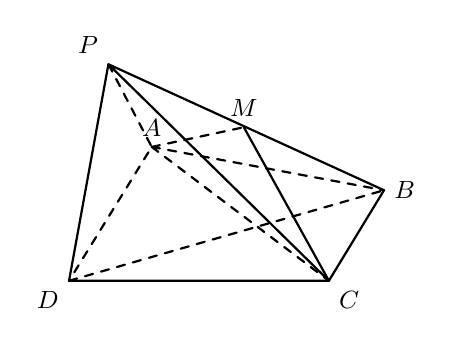
\begin{tikzpicture}[thick,line cap=round,line join=round,
  every node/.style={font=\small}]
  \coordinate (P) at (0,2.75);
  \coordinate (D) at (-.5,0);
  \coordinate (C) at (2.8,0);
  \coordinate (B) at (3.5,1.15);
  \coordinate (A) at (.55,1.7);
  \coordinate (M) at (1.72,1.95);
  \draw (P)--(D)--(C)--(B)--(P)--(C);
  \draw (M)--(C);
  \draw[dashed] (P)--(A)--(D) (A)--(B) (A)--(C) (A)--(M) (D)--(B);
  \node[above left] at (P) {$P$};
  \node[above] at (A) {$A$};
  \node[right] at (B) {$B$};
  \node[below right] at (C) {$C$};
  \node[below left] at (D) {$D$};
  \node[above] at (M) {$M$};
\end{tikzpicture}
\end{center}
\nopagebreak[4]
\Needspace{4\baselineskip}
\textbf{解析}

\gksubpart{（1）证明中点}

令 $E=AC\cap BD$。正方形的对角线互相平分，所以 $E$ 是 $BD$ 的中点。平面 $MAC$ 与平面 $PBD$ 的交线为 $ME$。由于 $PD\subset$ 平面 $PBD$ 且 $PD\parallel$ 平面 $MAC$，有 $PD\parallel ME$。

在三角形 $BPD$ 中，过 $BD$ 中点 $E$ 且平行于 $PD$ 的直线交 $BP$ 于 $M$，由中位线性质，$M$ 是 $PB$ 中点。

检查：$M$ 不能为 $P$，否则 $PD$ 与平面 $MAC$ 相交于 $P$；也不能为 $B$，否则平面 $MAC$ 就是底面而 $PD$ 交底面于 $D$。因此交线和中位线所用点均非退化。

\gksubpart{（2）二面角}

\Needspace{5\baselineskip}
采用以下自设直角坐标：

\nopagebreak[4]
\[A=(0,0,0),\quad D=(4,0,0),\quad B=(0,4,0),\quad C=(4,4,0).\]

\Needspace{5\baselineskip}
由平面 $PAD\perp$ 底面，$P$ 在平面 $y=0$ 内；由 $PA=PD$，$P$ 在 $AD$ 的垂直平分线上。设 $P=(2,0,h)$，选 $P$ 所在的一侧为 $z$ 正向，则

\nopagebreak[4]
\[4+h^2=6,\qquad h=\sqrt2.\]

故 $P=(2,0,\sqrt2)$，$M=(1,2,\sqrt2/2)$。

\Needspace{5\baselineskip}
为确定所求二面角而非其补角，将 $\overrightarrow{PA}$ 与 $\overrightarrow{PB}$ 分别投影到垂直于棱 $PD$ 的平面。记

\nopagebreak[4]
\[d=\overrightarrow{PD}=(2,0,-\sqrt2),\quad |d|^2=6.\]

\Needspace{5\baselineskip}
由于 $\overrightarrow{PA}\cdot d=\overrightarrow{PB}\cdot d=-2$，两投影向量为

\nopagebreak[4]
\[u=\overrightarrow{PA}+\tfrac13d=(-4/3,0,-4\sqrt2/3),\]
\nopagebreak[4]
\[v=\overrightarrow{PB}+\tfrac13d=(-4/3,4,-4\sqrt2/3).\]

\Needspace{5\baselineskip}
二者分别指向包含 $A$、$B$ 的半平面，且都垂直 $PD$，故它们的夹角就是所求二面角。计算

\nopagebreak[4]
\[u\cdot v=16/3,\quad |u|=4/\sqrt3,\quad |v|=8/\sqrt3,\]

\Needspace{5\baselineskip}
于是

\nopagebreak[4]
\[\cos\theta=\frac{u\cdot v}{|u||v|}=\frac12,\qquad\boxed{\theta=60^\circ}.\]

\gksubpart{（3）线面角}

\Needspace{5\baselineskip}
平面 $BDP$ 的方程是 $x+y+\sqrt2z=4$，可取法向量 $n=(1,1,\sqrt2)$。直线 $MC$ 的方向向量可取

\nopagebreak[4]
\[w=\overrightarrow{MC}=(3,2,-\sqrt2/2).\]

\Needspace{5\baselineskip}
记线面角为 $\varphi\in[0,\pi/2]$，则

\nopagebreak[4]
\[
\sin\varphi=\frac{|w\cdot n|}{|w||n|}
=\frac{4}{\sqrt{27/2}\cdot2}
=\boxed{\frac{2\sqrt6}{9}}.
\]

检查：$n$ 与 $\overrightarrow{PD}$、$\overrightarrow{PB}$ 内积均为零；$|n|=2$，$|w|^2=27/2$。所得正弦约 $0.5443$，位于 $[0,1]$。用 $M$ 的坐标计算平面 $MAC$ 的法向量 $(\sqrt2,-\sqrt2,2)$，与 $PD$ 方向内积为零，且 $P,D$ 均不在此平面，亦回证题设线面平行条件。

\gkanswer{答案（1）：$M$ 为 $PB$ 中点}

\gkanswer{答案（2）：$60^\circ$}

\gkanswer{答案（3）：$2\sqrt6/9$}

\end{answer}
\begin{answer}
\gksolhead{17}{}

\textbf{题目}：

为了研究一种新药的疗效，选 $100$ 名患者随机分成两组，每组各 $50$ 名，一组服药，另一组不服药。一段时间后，记录了两组患者的生理指标 $x$ 和 $y$ 的数据，并制成如图，其中“$\ast$”表示服药者，“$+$”表示未服药者。
\nopagebreak[4]
\begin{center}\begin{tikzpicture}[x=4.7cm,y=.048cm,>=stealth,thick,
  every node/.style={font=\small}]
  \draw[->] (0,35)--(1.08,35) node[right]{指标 $x$};
  \draw[->] (0,35)--(0,104) node[above]{指标 $y$};
  \node[below left] at (0,35) {$O$};
  \draw[dashed] (0,60)--(1.02,60);
  \draw[dashed] (.55,35)--(.55,101);
  \node[left] at (0,60) {$60$};
  \node[below] at (.55,35) {$1.7$};
  % Schematic symbol positions only: the source provides no individual data
  % coordinates. Fifty marks per group retain the source's visible count.
  \foreach \x/\y in {
    .12/89,.16/84,.20/78,.24/72,.28/65,.32/91,.36/83,.40/76,.44/69,.48/63,
    .10/58,.14/55,.18/52,.22/49,.26/46,.30/43,.34/40,.38/37,.42/34,.46/31,
    .18/88,.24/82,.30/75,.36/68,.42/61,.48/86,.50/79,.52/73,.54/66,.58/59,
    .08/95,.15/93,.23/90,.31/88,.39/85,.47/82,.11/75,.19/72,.27/70,.35/67,
    .43/64,.09/54,.17/51,.25/48,.33/45,.41/42,.49/39,.13/36,.21/33,.29/30}
    \node at (\x,\y) {$\ast$};
  \foreach \x/\y in {
    .57/86,.62/83,.67/80,.72/77,.77/74,.82/71,.87/68,.92/65,.97/62,.60/94,
    .65/91,.70/88,.75/85,.80/82,.85/79,.90/76,.95/73,.59/69,.64/66,.69/63,
    .74/60,.79/58,.84/56,.89/54,.94/52,.98/50,.61/97,.68/95,.76/93,.83/90,
    .91/88,.57/84,.63/81,.71/78,.78/75,.86/72,.93/70,.60/67,.67/64,.75/61,
    .82/59,.90/57,.96/55,.58/53,.66/51,.73/49,.81/47,.88/45,.95/43,.99/40}
    \node at (\x,\y) {$+$};
  \node[above left] at (.72,96) {$A$};
  \node[above left] at (.32,78) {$B$};
  \node[above right] at (.98,68) {$C$};
  \node[above left] at (.24,72) {$D$};
\end{tikzpicture}
\end{center}
\nopagebreak[4]
(1) 从服药的 $50$ 名患者中随机选出一人，求此人指标 $y$ 的值小于 $60$ 的概率；

(2) 从图中 $A,B,C,D$ 四人中随机选出两人，记 $\xi$ 为选出的两人中指标 $x$ 的值大于 $1.7$ 的人数，求 $\xi$ 的分布列和数学期望 $E(\xi)$；

(3) 试判断这 $100$ 名患者中服药者指标 $y$ 数据的方差与未服药者指标 $y$ 数据的方差的大小。（只需写出结论）

\Needspace{4\baselineskip}
\textbf{解析}

\gksubpart{（1）随机选一名服药者}

在 F17 放大图中，以星号中心是否严格低于 $y=60$ 的水平虚线逐点计数：左侧低于阈值的星号 14 个，右侧 1 个，总计 15 个。文本层辅助计数也给出 15，但结论已用渲染图复核。

\Needspace{5\baselineskip}
因此所求概率为

\nopagebreak[4]
\[\boxed{\frac{15}{50}=\frac3{10}}.\]

检查：分母是服药者 $50$ 人而非全部 $100$ 人；右下的加号不计入星号数；密集星号已放大分别计数，未将两枚近邻符号并为一枚。

\gksubpart{（2）分布列与期望}

\Needspace{5\baselineskip}
图中 $A,C$ 的 $x>1.7$，$B,D$ 的 $x<1.7$。从四人中等可能选两人，共 $\binom42=6$ 种。

\nopagebreak[4]
\[P(\xi=k)=\frac{\binom2k\binom2{2-k}}{\binom42},\qquad k=0,1,2.\]

\begin{center}
\begin{tabular}{llll}
\toprule
$\xi$ & 0 & 1 & 2 \\
\midrule
$P$ & $1/6$ & $2/3$ & $1/6$ \\
\bottomrule
\end{tabular}
\end{center}

\nopagebreak[4]
\[\boxed{E(\xi)=0\cdot\frac16+1\cdot\frac23+2\cdot\frac16=1}.\]

检查：概率和为 1；也可按每次选中“右侧人”的比例 $2/4$ 得期望 $2\times(2/4)=1$。四个有标签点均未落在阈值线上。

\gksubpart{（3）方差判断}

\Needspace{5\baselineskip}
候选结论为

\nopagebreak[4]
\[\boxed{\text{\text{服药者指标} }y\text{ \text{数据的方差大于未服药者指标} }y\text{ \text{数据的方差}。}}\]

依据是原图中星号在纵向较分散，较多分布于主体点群下方；加号则较集中于水平虚线上方的一条窄带。按题目“试判断”“只需写出结论”的要求作图形判断。

检查：比较的是纵坐标 $y$ 的离散程度，不是两组的 $x$ 分布或均值；不将“极差较大”当成所有数据情形下方差必大的定理。原图未给逐点精确数值，本稿不编造数值方差，此项同样保留 D 级待盲核属性。

\gkanswer{答案（1）：$3/10$}

\gkanswer{答案（2）：$P(\xi=0,1,2)=(1/6,2/3,1/6)$，$E(\xi)=1$}

\gkanswer{答案（3）：服药者的 $y$ 方差较大}

\end{answer}
\begin{answer}
\gksolhead{18}{}

\textbf{题目}：

已知抛物线 $C:y^2=2px$ 过点 $P(1,1)$。过点 $\left(0,\dfrac12\right)$ 作直线 $l$ 与抛物线 $C$ 交于不同的两点 $M,N$，过点 $M$ 作 $x$ 轴的垂线分别与直线 $OP,ON$ 交于点 $A,B$，其中 $O$ 为原点。

(1) 求抛物线 $C$ 的方程，并求其焦点坐标和准线方程；

(2) 求证：$A$ 为线段 $BM$ 的中点。

\Needspace{4\baselineskip}
\textbf{解析}

\gksubpart{（1）方程、焦点、准线}

\Needspace{5\baselineskip}
代入 $P(1,1)$ 得 $1=2p$，故 $p=1/2$，抛物线为

\nopagebreak[4]
\[\boxed{y^2=x}.\]

\Needspace{5\baselineskip}
对标准式 $y^2=2px$，焦点为 $(p/2,0)$、准线为 $x=-p/2$，所以

\nopagebreak[4]
\[\boxed{F=(1/4,0),\qquad x=-1/4}.\]

检查：此标准式的参数是 $2p$，不能把焦距误写成 $p$。

\gksubpart{（2）中点证明}

\Needspace{5\baselineskip}
若 $l$ 竖直，则只能是 $x=0$，与抛物线只有原点一个交点；若 $l$ 水平，则为 $y=1/2$，也只有一个交点。因此可设

\nopagebreak[4]
\[l:\ y=kx+1/2,\qquad k\ne0.\]

\Needspace{5\baselineskip}
设 $M=(y_1^2,y_1)$，$N=(y_2^2,y_2)$。联立得

\nopagebreak[4]
\[ky^2-y+1/2=0.\]

\Needspace{5\baselineskip}
由两个不同交点知 $y_1\ne y_2$；韦达定理给出

\nopagebreak[4]
\[y_1+y_2=1/k,\qquad y_1y_2=1/(2k),\]

\Needspace{5\baselineskip}
故

\nopagebreak[4]
\[y_1+y_2=2y_1y_2,\qquad y_1,y_2\ne0.\]

\Needspace{5\baselineskip}
直线 $OP$ 为 $y=x$，而 $ON$ 的斜率为 $1/y_2$。过 $M$ 的竖直线为 $x=y_1^2$，因此

\nopagebreak[4]
\[A=(y_1^2,y_1^2),\qquad B=(y_1^2,y_1^2/y_2).\]

\Needspace{5\baselineskip}
由上述韦达关系乘以 $y_1/y_2$，得

\nopagebreak[4]
\[\frac{y_1^2}{y_2}+y_1=2y_1^2.\]

所以 $y_A=(y_B+y_M)/2$，且三点横坐标相同，故 $A$ 为线段 $BM$ 的中点。

检查：两不同实交点对应 $1-2k>0$，且 $k\ne0$，排除了水平、竖直及相切情形。$y_2\ne0$ 保证 $ON$ 的斜率和 $B$ 坐标有定义。若 $B=M$，则 $y_1^2/y_2=y_1$，由 $y_1\ne0$ 得 $y_1=y_2$，与异点条件矛盾，故线段非退化，中点确位于端点之间。

\gkanswer{答案（1）：$y^2=x$，焦点 $(1/4,0)$，准线 $x=-1/4$}

\gkanswer{答案（2）：$A$ 为 $BM$ 中点}

\end{answer}
\begin{answer}
\gksolhead{19}{}

\textbf{题目}：

已知函数 $f(x)=\mathrm e^x\cos x-x$。

(1) 求曲线 $y=f(x)$ 在点 $(0,f(0))$ 处的切线方程；

(2) 求函数 $f(x)$ 在区间 $\left[0,\dfrac\pi2\right]$ 上的最大值和最小值。

\Needspace{4\baselineskip}
\textbf{解析}

\gksubpart{(1)}
\Needspace{5\baselineskip}
（1）$f(0)=1$，

\nopagebreak[4]
\[f'(x)=\mathrm e^x(\cos x-\sin x)-1,\qquad f'(0)=0.\]

\Needspace{5\baselineskip}
切线为

\nopagebreak[4]
\[\boxed{y=1}.\]

\gksubpart{(2)}
\Needspace{5\baselineskip}
（2）继续求导：

\nopagebreak[4]
\[f''(x)=-2\mathrm e^x\sin x.\]

\Needspace{5\baselineskip}
在 $0<x\leqslant\pi/2$ 上 $f''(x)<0$，所以 $f'(x)$ 在所给区间上严格递减；由 $f'(0)=0$，得 $f'(x)<0$（$0<x\leqslant\pi/2$）。因此 $f$ 在 $[0,\pi/2]$ 上严格递减。

\nopagebreak[4]
\[\boxed{f_{\max}=f(0)=1,\qquad f_{\min}=f(\pi/2)=-\pi/2}.\]

检查：函数在闭区间上连续，两端点均包含；$x=0$ 处导数为零不妨碍整体严格递减，不能据此另添内部极值。$\cos(\pi/2)=0$，端点代入正确。

\gkanswer{答案（1）：$y=1$}

\gkanswer{答案（2）：最大值 $1$，最小值 $-\pi/2$}

\end{answer}
\begin{answer}
\gksolhead{20}{}

\textbf{题目}：

\Needspace{5\baselineskip}
设 $\{a_n\}$ 和 $\{b_n\}$ 是两个等差数列，记

\nopagebreak[4]
\[
c_n=\max\{b_1-a_1n,\ b_2-a_2n,\ \cdots,\ b_n-a_nn\}\qquad(n=1,2,3,\cdots),
\]

其中 $\max\{x_1,x_2,\cdots,x_s\}$ 表示 $x_1,x_2,\cdots,x_s$ 这 $s$ 个数中最大的数。

(1) 若 $a_n=n$，$b_n=2n-1$，求 $c_1,c_2,c_3$ 的值，并证明 $\{c_n\}$ 是等差数列；

(2) 证明：或者对任意正数 $M$，存在正整数 $m$，当 $n\geqslant m$ 时，$\dfrac{c_n}{n}>M$；或者存在正整数 $m$，使得 $c_m,c_{m+1},c_{m+2},\cdots$ 是等差数列。

\Needspace{4\baselineskip}
\textbf{解析}

定义中 $a_i n$ 表示乘积 $a_i\cdot n$，其中取最大值时 $n$ 固定、$i=1,\ldots,n$ 变化。

\gksubpart{（1）具体数列}

\Needspace{5\baselineskip}
当 $a_i=i,b_i=2i-1$ 时，

\nopagebreak[4]
\[b_i-na_i=(2-n)i-1.\]

$n=1$ 时只有 $i=1$，得 $c_1=0$；$n=2$ 时各项均为 $-1$，得 $c_2=-1$；$n=3$ 时最大值在 $i=1$ 取得，得 $c_3=-2$。

\Needspace{5\baselineskip}
一般地，$n\geqslant2$ 时系数 $2-n\leqslant0$，最大值可以在 $i=1$ 取得，因此 $c_n=1-n$。这个公式对 $n=1$ 也成立，所以

\nopagebreak[4]
\[\boxed{c_n=1-n},\]

即 $\{c_n\}$ 是首项为 $0$、公差为 $-1$ 的等差数列。

检查：$n=2$ 时最大项不唯一，但最大值唯一，不影响通项。

\gksubpart{（2）一般情形的完整分类}

\Needspace{5\baselineskip}
设

\nopagebreak[4]
\[a_i=A+(i-1)d,\qquad b_i=B+(i-1)e,\]

\Needspace{5\baselineskip}
其中 $A=a_1,B=b_1$，$d,e$ 分别为两个等差数列的公差。对固定 $n$，

\nopagebreak[4]
\[b_i-na_i=B-nA+(i-1)(e-nd).\]

\Needspace{5\baselineskip}
这是关于 $i$ 的一次式，因此最大值必在端点取得（斜率为零时所有项相等）：

\nopagebreak[4]
\[\boxed{c_n=B-nA+(n-1)\max\{0,e-nd\}}.\tag{*}\]

\Needspace{5\baselineskip}
\textbf{情形一：$d<0$。} 存在正整数 $m_0$，使 $n\geqslant m_0$ 时 $e-nd>0$。于是由 $(*)$，

\nopagebreak[4]
\[c_n=-dn^2+(e+d-A)n+B-e,\]

\nopagebreak[4]
\[\frac{c_n}{n}=-dn+(e+d-A)+\frac{B-e}{n}.\]

\Needspace{5\baselineskip}
因 $-d>0$，此式趋于 $+\infty$。具体地，给定任意 $M>0$，取正整数 $m\geqslant m_0$ 且

\nopagebreak[4]
\[m>\frac{M+|e+d-A|+|B-e|}{-d}.\]

\Needspace{5\baselineskip}
则对一切 $n\geqslant m$（因 $n\geqslant1$），

\nopagebreak[4]
\[\frac{c_n}{n}\geqslant-dn-|e+d-A|-|B-e|>M.\]

这正是题目的第一种结论。

\Needspace{5\baselineskip}
\textbf{情形二：$d>0$。} 取正整数 $m$ 使 $md\geqslant e$，则 $n\geqslant m$ 时 $e-nd\leqslant0$。由 $(*)$，

\nopagebreak[4]
\[c_n=B-An\qquad(n\geqslant m).\]

故 $c_m,c_{m+1},\ldots$ 是公差为 $-A$ 的等差数列，满足第二种结论。

\Needspace{5\baselineskip}
\textbf{情形三：$d=0$。} 此时 $e-nd=e$ 恒定。若 $e\leqslant0$，则 $c_n=B-An$；若 $e>0$，则

\nopagebreak[4]
\[c_n=B-An+(n-1)e=(e-A)n+B-e.\]

两者从 $n=1$ 起就是等差数列，取 $m=1$ 即满足第二种结论。

三类覆盖全部实数公差 $d$，命题得证。

检查：$e-nd=0$ 的临界点已包含于非正分支，两端点给同一最大值；$n=1$ 时 $(*)$ 自动给出 $B-A$。证明保留“对任意 $M$，从某项起所有 $n$ 都满足”的量词，未将其弱化为存在若干趋大的子列项。若数列尾部为等差数列，则 $c_n/n$ 趋于有限的尾部公差，故不会同时满足第一分支的趋于 $+\infty$。

\gkanswer{答案（1）：$c_1=0,c_2=-1,c_3=-2,c_n=1-n$}

\gkanswer{答案（2）：按 $\{a_n\}$ 公差的正、负、零分类证明}

\end{answer}